\documentclass[11pt, twoside, pdftex]{article}

% This include all the settings that we should use for the document
\newcommand{\PDFTitle}{Getting Started with Intel's DE-Series Boards}
\newcommand{\commonPath}{../../../Tutorials/Common}
\input{\commonPath/Docs/defaulttext.tex}
\input{\commonPath/Docs/preamble.tex}
\widowpenalty 10000

%%%%%%%%%%%%%%%%%%%%%%%%%

% Add title
\newcommand{\doctitle}{DESim Installation Guide}
\newcommand{\dochead}{DESim Installation Guide}
% Usually no need to change these two lines

\title{\fontfamily{phv}\selectfont{\doctitle} }
\chead{ \small{\textsc{\bfseries \dochead} } }
% Customizations
%%%%%%%%%%%%%%%%%%%%%%%%%
% Allows multiple figures per page

\renewcommand\floatpagefraction{.9}
\renewcommand\topfraction{.9}
\renewcommand\bottomfraction{.9}
\renewcommand\textfraction{.1}   
\setcounter{totalnumber}{50}
\setcounter{topnumber}{50}
\setcounter{bottomnumber}{50}
\raggedbottom
\usepackage{enumitem}
\setlist{nolistsep}

\usepackage{tikz}
\usetikzlibrary{shadows}

\newcommand\keystroke[1]{
  \tikz[baseline=(key.base)]
    \node[
      draw,
      fill=white,
      drop shadow={shadow xshift=0.25ex,shadow yshift=-0.25ex,fill=black,opacity=0.35},
      rectangle,
      rounded corners=2pt,
      inner xsep=3pt,
      inner ysep=0.5pt,
      line width=0.5pt,
      font=\scriptsize\sffamily
  ](key) {#1\strut}
  ;
}

%%%%%%%%%%%%%%%%%%
%%% DOCUMENT START
%\begin{document}
\begin{document}
\begin{table}
    \centering
    \begin{tabular}{p{5cm}p{4cm}}
        \hspace{-3cm}
        &
        \raisebox{1\height}{\parbox[h]{0.5\textwidth}{\Large\fontfamily{phv}\selectfont{\textsf{\doctitle}}}}
    \end{tabular}
    \label{tab:logo}
\end{table}

\colorbox[rgb]{0,0.384,0.816}{\parbox[h]{\textwidth}{\color{white}\textsf{\textit{\textBar}}}}

\thispagestyle{plain}

\definecolor{AppleGreen}{rgb}{0.55, 0.71, 0.0}
\newcommand{\green}[1]{{\color{AppleGreen}\sf{#1}}}
\newcommand{\red}[1]{{\color{red}\sf{#1}}}


\section{Introduction}

This tutorial shows you how to download and install the {\it DESim} application
on a computer that is running a Microsoft Windows or Ubuntu operating systems.  
To perform the steps given below you will need to have 
access to the Internet, and have the required permissions to install application software.

We do not give detailed instructions in this document for using the {\it DESim} application, 
but only show how to install it. Separate instructions for using the {\it DESim} application 
are provided in the tutorial called 
\href{https://github.com/fpgacademy/DESim/releases/download/v2.0/DESim\_tutorial.pdf}
{Using the DESim Software with Verilog/VHDL Code}.
Before using the {\it DESim} application it is necessary to install either the {\it ModelSim} 
or {\it Questa} simulation software. This version of the {\it DESim} application was built for:
\begin{itemize}
	\item {\it ModelSim-Intel FPGA} edition software v10.5b which comes with the 
{\it Quartus Prime} software v19.1. 
	\item {\it Questa-Intel FPGA} edition software v2021.2 which comes
		with the 
{\it Quartus Prime} software v21.1. 
\end{itemize}
Instructions for installing the {\it ModelSim} and {\it Questa} applications are
provided in the tutorials  {\it Using the ModelSim-Intel FPGA Simulator with Verilog/VHDL
Testbenches} and {\it Using the Questa-Intel FPGA Simulator with Verilog/VHDL Testbenches}, 
respectively, available on \href{https://www.fpgacademy.org/tutorials.html}{FPGAcademy.org}. 

\section{Getting Started}

The discussion below assumes that you are using the Google {\it Chrome} Internet Browser to
navigate on the Internet.  If you are using a different browser application, then you may
notice some minor discrepancies from some of the material presented below. 

You can download the {\it DESim} software installer from its repository on {\it GitHub}. 
Open your Internet browser and navigate to \url{https://github.com/fpgacademy/DESim/releases}.
This action opens the repository's \texttt{Releases} page, part of which is shown in 
Figure~\ref{fig:release}

The {\it DESim} repository includes the source-code 
for the application. You can browse through this code if interested, but it is not necessary to
do so.

If using the Microsoft Windows operating system, read section~\ref{sec:win_inst}. If using the
Ubuntu operating system, jump to section~\ref{sec:ubuntu_inst}. After read either of those sections,
continue reading at section~\ref{sec:env}

\subsection{Windows Installation} \label{sec:win_inst}

Click on the filename {\it desim\_setup.exe}, as illustrated in Figure~\ref{fig:release},
which downloads this file to your computer. You may be presented with a
warning message in your browser, because the file that you are downloading is an 
{\it executable program}. Make the appropriate selections in your browser to keep the downloaded
file so that it is saved onto your computer.

\begin{figure}[h]
	\begin{center}
        \setlength{\fboxsep}{0pt}
        \fbox{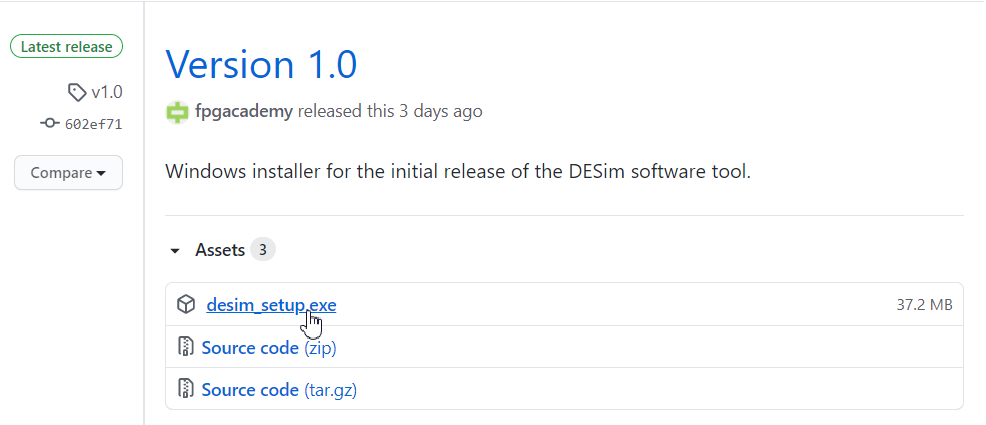
\includegraphics[scale=0.75]{figures/GitHub_releases.png}}
	\end{center}
          \caption{The \texttt{Releases} page for the {\it DESim} repository.}
	\label{fig:release}
\end{figure}

The {\it desim\_setup.exe} file is the {\it installer} program for the {\it DESim}
application. Open this file (execute the program) to reach the \texttt{Welcome} screen 
shown in Figure~\ref{fig:welcome}. Click \texttt{Next} to see the {\it License Agreement}
for the {\it DESim} application, and then click \texttt{I Agree} if you accept the terms of 
the license. If you do not accept the terms of the agreement, then the installer will
exit. Click \texttt{Next} to reach the screen displayed in Figure~\ref{fig:install}.

\begin{figure}[h]
	\begin{center}
        \setlength{\fboxsep}{0pt}
        \fbox{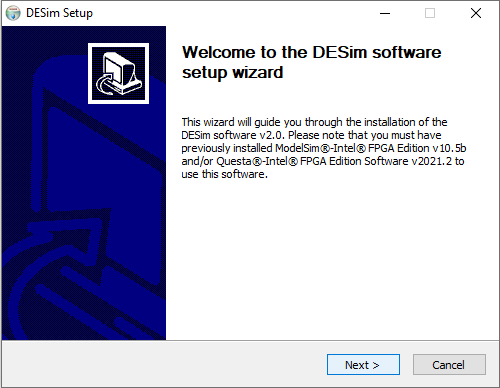
\includegraphics[scale=.75]{figures/welcome.png}}
	\end{center}
          \caption{The first screen of the {\it DESim} installer.}
	\label{fig:welcome}
\end{figure}

As shown in Figure~\ref{fig:install}, you can specify an installation folder. In the discussion
below, we assume that you have accepted the default location (\texttt{C:$\backslash$DESim}),
but you can change this selection. Click the \texttt{Install} button. 
During the installation process you have the option of placing an icon onto your
\texttt{Desktop} for this application. This icon provides an easy way to run the {\it DESim}
application, and so is recommended. 

\begin{figure}[h]
	\begin{center}
        \setlength{\fboxsep}{0pt}
        \fbox{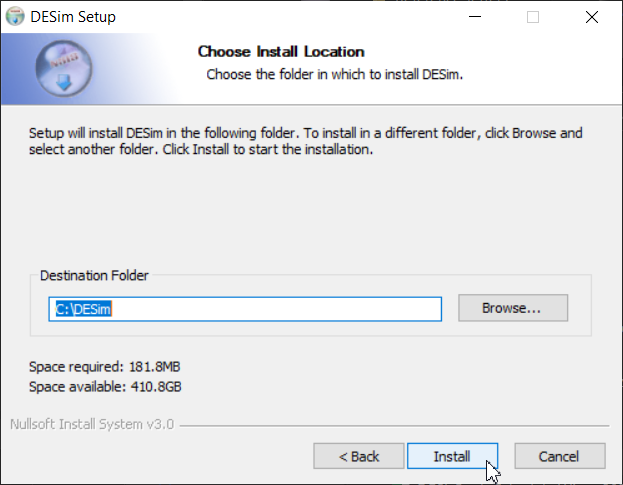
\includegraphics[scale=.75]{figures/install.png}}
	\end{center}
          \caption{Installing the {\it DESim} application.}
	\label{fig:install}
\end{figure}

The \texttt{C:$\backslash$DESim} folder created in the installation process
contains the {\it DESim} software and some
example projects (called {\it demos}). Start the {\it DESim} application by double-clicking its
{\it icon} on your \texttt{Desktop}, or by selecting {\it DESim} from the 
{\it Windows Start} menu. Alternatively, you can use \texttt{File Explorer} to run the 
{\it DESim} application by navigating to the \texttt{C:$\backslash$DESim} folder, 
right-clicking on the {\it batch} file \texttt{DESim\_run.bat}, as illustrated in 
Figure~\ref{fig:open}, and then selecting \texttt{Open} (or, you can double-click on the 
batch file to open it).

\begin{figure}[h]
	\begin{center}
            \setlength{\fboxsep}{0pt}
            \fbox{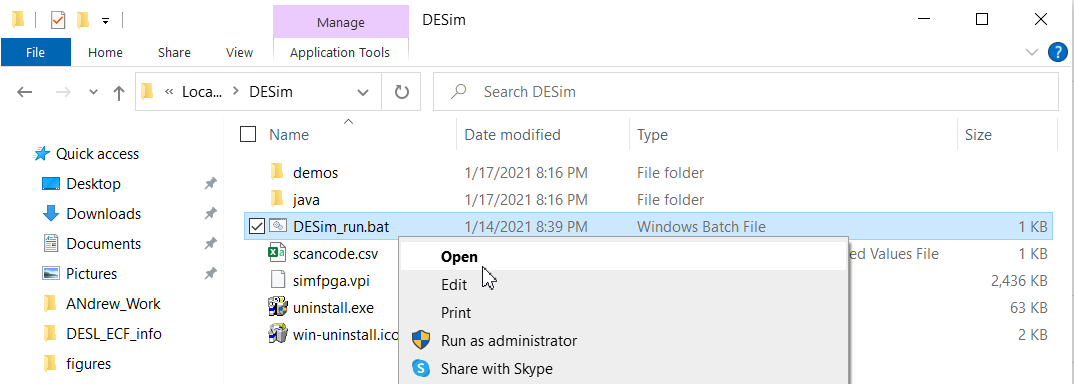
\includegraphics[width = 1\textwidth]{figures/DESim_open_local.png}}
	\end{center}
          \caption{Starting the {\it DESim} application under Windows.}
	\label{fig:open}
\end{figure}

\subsection{Linux Installation} \label{sec:ubuntu_inst}

Click on the filename {\it desim.tar.gz}, as illustrated in Figure~\ref{fig:release},
which downloads this file to your computer. 
Extract the contents of the tarball to a folder, such has \texttt{$\sim$/DESim}. This
newly created directory contains the {\it DESim} software and some
example projects (called {\it demos}). Start the {\it DESim} application by running the 
\texttt{./DESim.sh} script. As shown in Figure~\ref{fig:run_linux}, this can be done by: 
\begin{enumerate}
	\item Opening a terminal window using keys \keystroke{Ctrl} + \keystroke{Alt} + \keystroke{T}
	\item Navigating to the newly create directory: `\texttt{cd $\sim$/DESim}'
	\item Executing the shell script: `\texttt{./DESim.sh}'
\end{enumerate}

\begin{figure}[h]
	\begin{center}
            \setlength{\fboxsep}{0pt}
            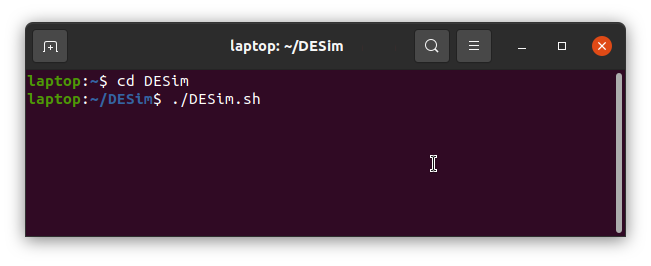
\includegraphics[width = 1\textwidth]{figures/DESim_run_linux.png}
	\end{center}
          \caption{Starting the {\it DESim} application under Linux.}
	\label{fig:run_linux}
\end{figure}

\subsection{Enviroment configuration} \label{sec:env}

The {\it DESim} software requires that the simulation software's executables are in your 
{\it PATH} environment variable. Additionally, some versions of the simulation software require a 
license file. If the installed simulation software on your computer does require a license file, 
the path to license file must be properly specified by an {\it LM\_LICENSE\_FILE} environment variable. 
If these environment variables are not set correctly on your computer, appropriate values can be supplied
as command-line arguments to the {\it DESim} software. To add these command-line arguments,
modify the \texttt{DESim.bat} (Windows) or \texttt{DESim.sh} (Linux) as described in those files.


\section{Running DESim}

You should now see the {\it DESim} graphical user interface (GUI),
illustrated in Figure~\ref{fig:GUI}. It should show the message
``\green{The server is running...}'' near the top of the {\it message pane} in the GUI.

\begin{figure}[h]
	\begin{center}
		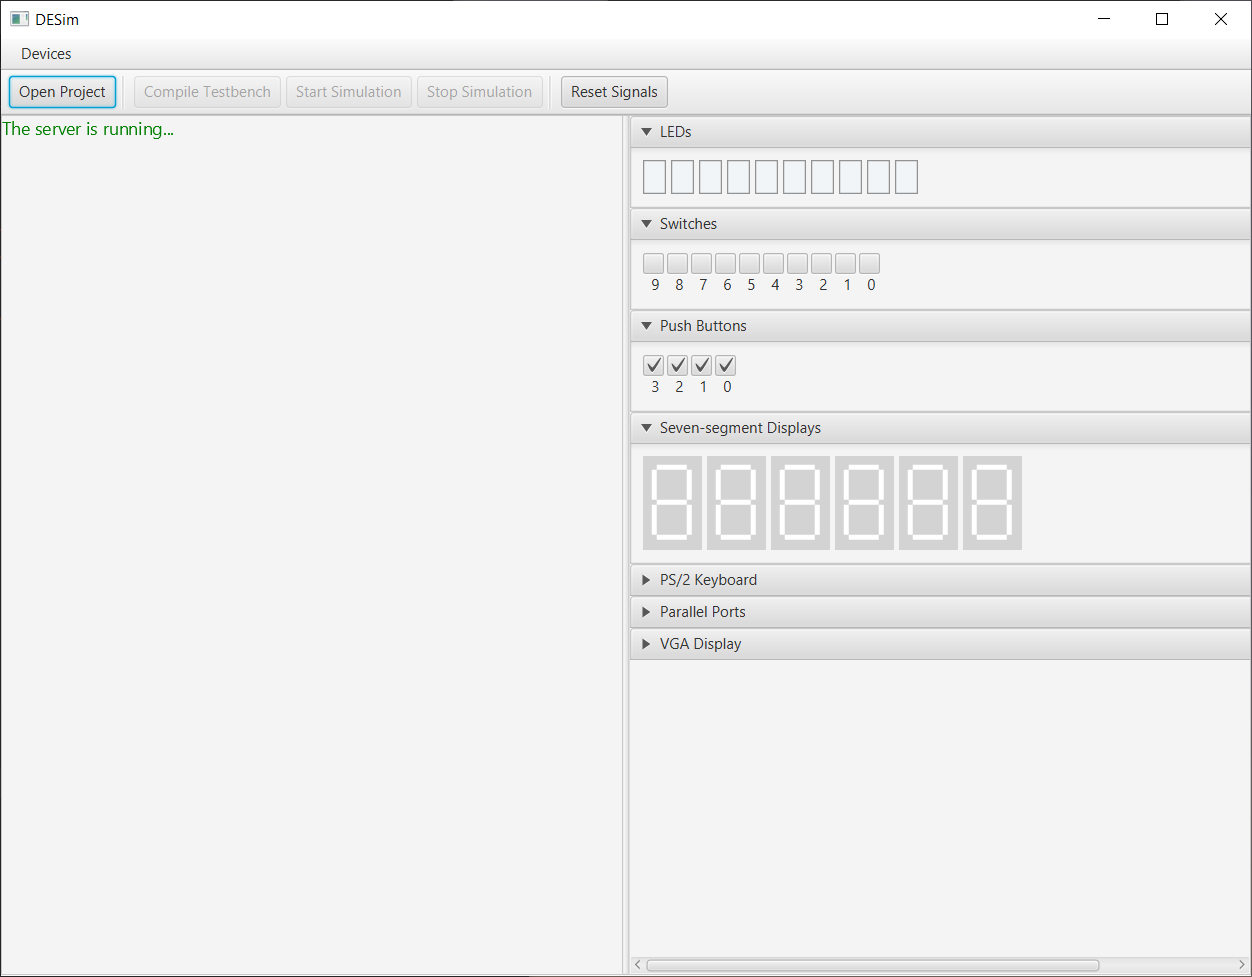
\includegraphics[width = \textwidth]{figures/DESim_GUI.png}
	\end{center}
          \caption{The {\it DESim} window.}
	\label{fig:GUI}
\end{figure}


To ensure that the {\it DESim} application can communicate with the {\it ModelSim} simulator, you
may wish to try out one (or more) of the {\it demo} projects that come with {\it DESim}. As
an example, click the \texttt{Open Project} button in the {\it DESim} GUI and then navigate into
the \texttt{demos} folder. Next, click to select the appropriate folder, either \texttt{modelsim} 
or \texttt{questa}, depending on which simulation software is installed. Then, click to select 
either the \texttt{verilog} or \texttt{vhdl} folder for examples written in your preferred 
hardware description language (HDL). In Windows, click to select the folder named \texttt{LED\_HEX} 
and then click the \texttt{Select Folder} button, as illustrated in Figure~\ref{fig:demos_windows}.
In Linux, navigate to the folder named \texttt{LED\_HEX} and then click the
\texttt{Open} button, as illustrated in Figure~\ref{fig:demos_linux}.
In the example, we have chosen the {\it Questa} simulator and the {\it Verilog} HDL. 
The navigation bar in the dialog will look different, if you chosen other options.

\begin{figure}[h]
	\begin{center}
        \setlength{\fboxsep}{0pt}
        \fbox{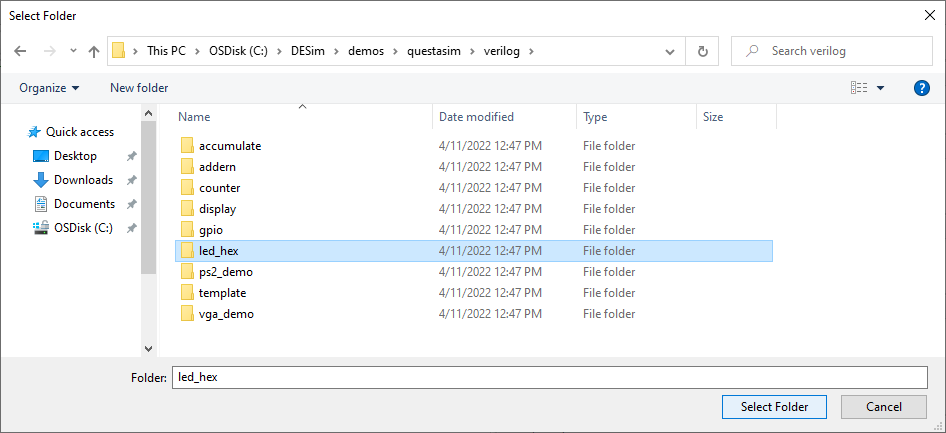
\includegraphics[width = .9\textwidth]{figures/DESim_project_windows.png}}
	\end{center}
    \caption{Opening a sample project in the \texttt{demos} folder under Windows.}
	\label{fig:demos_windows}
\end{figure}

\floatstyle{plain}
\restylefloat{figure}
\begin{figure}[h]
	\begin{center}
        \setlength{\fboxsep}{0pt}
        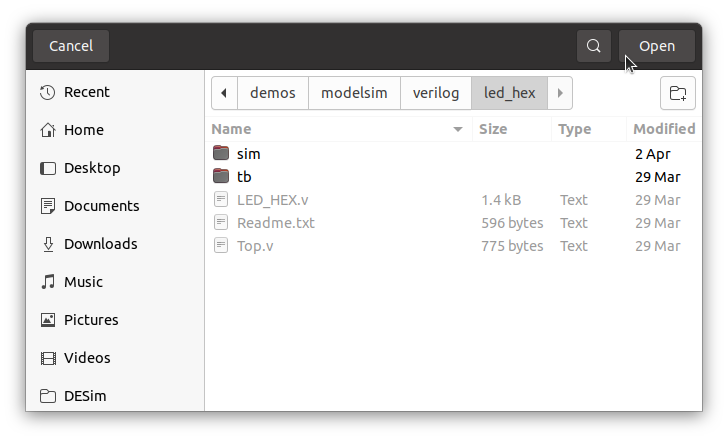
\includegraphics[width = .9\textwidth]{figures/DESim_project_linux.png}
	\end{center}
    \caption{Opening a sample project in the \texttt{demos} folder under Linux.}
	\label{fig:demos_linux}
\end{figure}

Click the \texttt{Compile Testbench} button in {\it DESim}. As shown in 
Figure~\ref{fig:compile}, the {\it Questa} simulation software is executed to compile the
Verilog code for the sample project, and the compilation messages that are produced by 
{\it Questa} are displayed in the {\it DESim} message pane.

In the {\it DESim} window, click the \texttt{Start Simulation} button, which starts the
{\it Questa} simulation software. As illustrated in Figure~\ref{fig:sim}, any messages
produced by {\it Questa} are displayed in the message pane of the {\it DESim} window. 
To make your display look like the one in the figure, in the {\it DESim} GUI click on 
the \texttt{Switch} with index number
\texttt{6}, which causes the corresponding \texttt{LED} to turn \red{red}. To activate the
\texttt{Seven-segment Display} output you have to reset the \texttt{LED\_HEX} circuit. To
do this, click on \texttt{Push Button} \texttt{0} to press it, and then click again to
release this button. 
To learn about the features of the \texttt{LED\_HEX} project, you can follow 
the instructions in its {\it Readme.txt} file, shown in Figure~\ref{fig:readme}, and/or 
read through the HDL file. The Verilog source-code file \texttt{LED\_HEX.v} is displayed in 
Figure~\ref{fig:verilog_top}. The VHDL source-code file \texttt{LED\_HEX.vhd} is displayed in 
Figure~\ref{fig:vhdl_top}. Each example included with {\it DESim} has its own {\it Readme.txt} 
file and HDL files, which can be read to learn more about them.
%These files can be found
%using the Microsoft Windows \texttt{File Explorer} in the \texttt{LED\_HEX} folder.

You can stop the simulation by clicking the \texttt{Stop Simulation} button 
in the {\it DESim} GUI. To close the {\it DESim} program click the $\times$ in 
the upper-right corner of the window.    

\begin{figure}[h]
	\begin{center}
        \setlength{\fboxsep}{0pt}
        \fbox{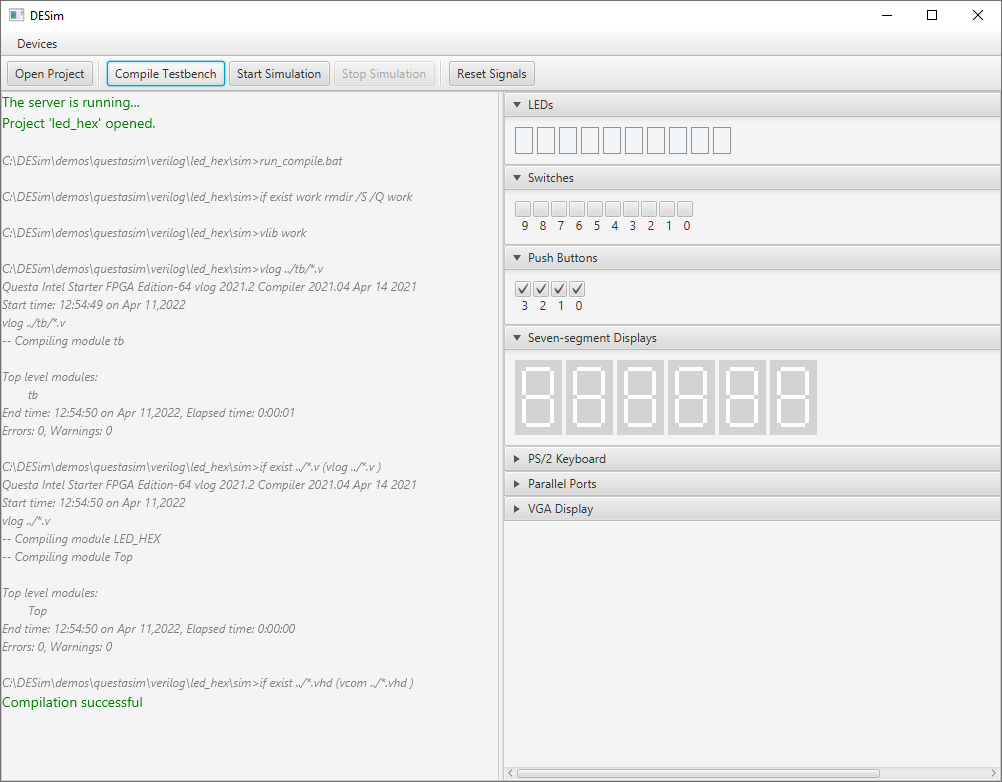
\includegraphics[width = .9\textwidth]{figures/DESim_compile.png}}
	\end{center}
          \caption{Compiling the sample project.}
	\label{fig:compile}
\end{figure}

\begin{figure}[h]
	\begin{center}
        \setlength{\fboxsep}{0pt}
        \fbox{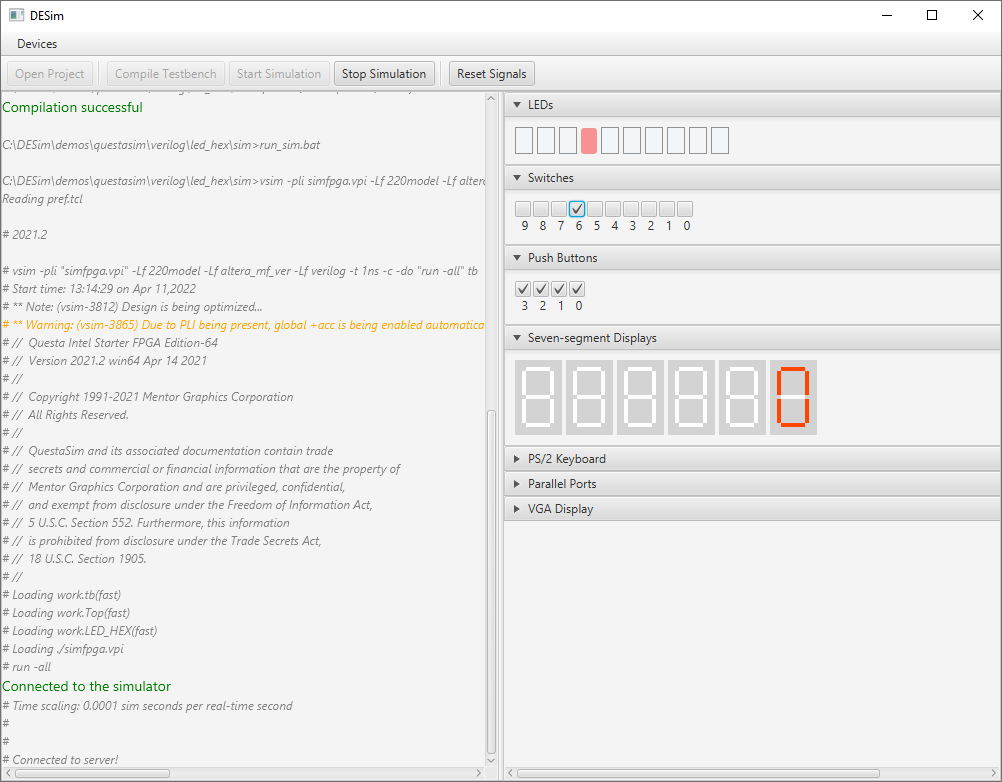
\includegraphics[width = \textwidth]{figures/DESim_simulate.png}}
	\end{center}
          \caption{Simulating the sample project.}
	\label{fig:sim}
\end{figure}


\begin{figure}[h]
\begin{center}
\begin{minipage}[t]{16 cm}
	\lstinputlisting[numbers=none]{../../demos/led_hex/Readme.txt}
\end{minipage}
	\caption{The {\it Readme.txt} file for the \texttt{LED\_HEX} project.}
	\label{fig:readme}
\end{center}
\end{figure}

\begin{figure}[h]
\begin{center}
\begin{minipage}[t]{15 cm}
	\lstinputlisting[language=Verilog,numbers=none,firstline=12]{../../demos/led_hex/led_hex.v}
\end{minipage}
	\caption{The Verilog source-code file \texttt{LED\_HEX.v}.}
	\label{fig:verilog_top}
\end{center}
\end{figure}

\begin{figure}[h]
\begin{center}
\begin{minipage}[t]{15 cm}
	\lstinputlisting[language=VHDL,numbers=none,firstline=13]{../../demos/led_hex/led_hex.vhd}
\end{minipage}
	\caption{The VHDL source-code file \texttt{LED\_HEX.vhd}.}
	\label{fig:vhdl_top}
\end{center}
\end{figure}


\input{\commonPath/Docs/copyright.tex}

\end{document}
